\begin{refsection}
\chapter*{De l'information au savoir}
\markboth{Introduction --- De l'information au savoir}{Introduction --- De l'information au savoir}
\addcontentsline{toc}{chapter}{Introduction --- De l'information au savoir}

Un des enjeux majeur de la science, a été de tout temps, la recherche de la véracité des théories. En effet, une théorie communément acceptée, permet d'aboutir à un savoir transmissible. Pour cela, il est indispensable de procéder avec méthode.

Dès l'antiquité, la nécessité de démontrer, les causes expliquant avec certitudes les conséquences, émerge avec Aristote (384 - 322 av. J.-C.). À travers Alhazen (965 - 1039) l'idée pris forme autour de méthodes expérimentales et reproductibles. Son traité \citetitle{Alhazen1572} détaille précisément ces expériences, ainsi tout lecteur, parvient aux mêmes conclusions. Ses méthodes furent reprises en Occident par Roger Baconn (1220 - 1294). Cette démarche expérimentale décrit les prémisses d'une méthode scientifique. Elle a évolué tout au long de l'histoire, afin d'être rigoureuse, vérifiable et reproductible.

Ainsi, le trio observation, modélisation et expérimentation s'est imposé comme fondement d'une démarche scientifique. Ces trois paramètres permettent d'amener les éléments de confiance et d'impartialité nécessaire pour vérifier une théorie.

\citation{
    Nous estimons posséder la science d'une chose d'une manière absolue, ... quand nous croyons que nous connaissons la cause par laquelle la chose est, que nous savons que cette cause est celle de la chose, et qu'en outre il n'est pas possible que la chose soit autre qu'elle n'est.}{Aristote}[(Seconds Analytiques I, 31, 88a, 4)]


Cependant l'explosion des théories a rendu cette démarche fastidieuse. En effet, elle nécessite une intervention humaine minutieuse afin de vérifier toutes les observations vis-à-vis du savoir. Par exemple le nombre de communications scientifique, est estimé à plus 50 millions \cite{LEAP:LEAP0509}. C'est autant d'information à vérifier les unes par rapports aux autres. On peut légitimement se demander, s'il est possible de confronter l'ensemble des observations et théories, vis-à-vis du savoir. Ceci permettrais d'évaluer nos certitudes et produire in-fine de nouveaux savoir.

Les observations sont des éléments précurseurs à la connaissance, elles sont utilisées pour émettre des théories. L'émergence des technologies de l'information nous permettent de récupérer un nombre d'observations toujours plus grand. Cet évènement ouvre de nouvelles possibilités. C'est l'ère du \textit{"Big Data"}.

Ainsi, notre capacité à générer des informations ne cesse d'augmenter. Elle dépasse largement, les capacités humaines nécessaires à l'expertise de ces informations. En effet, les méthodes informatisées génèrent continuellement et rapidement des données. De plus les super-calculateurs, support de ces méthodes informatisées, deviennent de plus en plus rapide, augmentant les capacités de traitement de l'information. De tels outils, se démocratisent dans tous les domaines de la science. Avec l'essor de ces nouvelles technologies, la barrière entre information et savoir devient de plus en plus flou.

\note{
    L'origine du mot science, vient du latin \textit{"scientia"} désignant le savoir.
    
    La connaissance est propre à une personne. À contrario le savoir est transmissible.
    
    De nombreuses langues, comme l'anglais ne possède pas de mot pour différencier savoir et connaissance. En effet, dans les deux cas on utilise \textit{"knowledge"}. Afin de marquer la nuance, on retrouve l'expression \textit{"certified knowledge"} pour le savoir et \textit{"learning by doing"} pour la connaissance.
}

Ces données produites par la recherche sont entreposées dans des bases de données. Certains entrepôts de données partagent un même champs de savoir. Toutefois elles diffèrent par leurs contenu. L'ensemble des entrepôts d'un même champ de savoir constitue une vision complètes des informations observées. Toutefois, cet ensemble d'information ne garantie pas la couverture de toutes les régions du savoir. De plus, unitairement ces bases de données peuvent veiller à la consistance de leurs données. Mais bien souvent ils ne disposent pas d'outils de vérification inter-base de donnée. Pour cette raison l'utilisation d'information provenant de plusieurs entrepôt peut mener à des contradictions. 

Il est indubitable que nous ne pouvons plus mener des recherches sur des vastes domaines comme "la Biologie", "les Mathématiques", "la Physique". Les connaissances à maitriser sont trop nombreuses. Les chercheurs, se spécialisent de plus en plus afin de maitriser un domaine toujours plus pointu. Malgré tous ces efforts, dans de nombreux domaines, il nous est impossible d'appréhender tous les travaux liés. Or ces connaissances, nous sont non seulement
importantes pour valider ou non les prédictions ; mais il nous est également nécessaire d'élargir nos connaissances, hors de notre domaine d'expertise pour mieux le comprendre en retour.(trop long)

\citation{La séparation des savoirs, la spécialisation en domaine isolé nuit considérablement au développement de la recherche.}{Jacques Le Goff}[Le Monde de l'éducation - Mai 2000]

Rechercher la véracité des connaissances, nécessite de pouvoir représenter nos théories puis de les confrontés aux différentes prédictions et expectations. Ce travail ne peut plus être réalisé uniquement par l'Homme, il doit être assisté par des méthodes informatisées capable de répondre aux défis d'aujourd'hui et de demain.

Ce constat se vérifie en biologie, avec l'avènement des séquenceurs nouvelles générations. Le séquençage des organismes est devenu abordable et rapide. Ainsi la communauté scientifique à initier de vaste projet de séquençage du monde vivant. Ces projets permettent d'avoir le code génétique, également nommée séquence \gls{ADN}. Cette chaîne \gls{ADN} peut être composé de quelques milliers à plusieurs centaines de millions de paires de bases nucléiques. Selon l'ordonnancement des bases nucléotidiques, des régions appelées gènes, procurent des fonctionnalités à l'organisme. Ainsi, L'\gls{ADN} est un point départ pour l'étude et la compréhension des fonctionnalités inscrite dans le vivant.

\begin{figure}[!h]
    \centering
    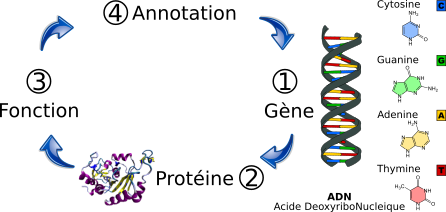
\includegraphics{img/simple_annotation_process_numéroté.png}
    \caption{Vue globale du gène à l'annotation }
    \label{fig:glob_annotation}
\end{figure}

Des outils bio-informatiques analysent ces séquences afin de prédire les régions géniques et leurs fonctions dans l'organisme (voir figure \ref{fig:glob_annotation}). Selon les organismes, le nombre de gène varie de quelques millier à plusieurs dizaines de milliers de gènes. Ainsi, parmis le million voire milliard de paire de base d'\gls{ADN}, il faut identifier tous les gènes. Par conséquent, l'expertise humaine d'un génome est un défi en soi. Ces recherches se sont intensifiées et complexifiées, comme l'étude de 100 000 génomes d'organismes pathogènes \cite{100kfoodborne}, ou encore sur les eco-systèmes poly-microbiens présent sur l'Homme \cite{hmp}.

Pour se faire des outils bio-informatiques ont automatisé le traitement de l'information issue des séquenceurs afin de traiter un nombre d'organisme toujours plus grand. Ces outils, alimentés continuellement en nouveaux génomes, ont amplifié le déluge d'information. Dans le domaine de l'annotation fonctionnelle, moins d'un pour cent des données ont pu être vérifiées (au regard des statistiques publiés par UniProt et SwissProt en 2017 \parencites{uniprot_stat}{expasy_stat} ). Ce fossé entre information de confiance et prédiction s'accélère car il est plus rapide de produire de l'information que de la vérifier.

Or les prédicteurs automatiques de fonctions géniques ne sont pas fiables. En effet, 30\% des annotations fonctionnelles seraient incorrectes, voire 80\% dans certaines familles de protéines \parencites{devos2001intrinsic}{schnoes2009annotation}. Ces séquences incorrectement annotées sont ensuite propagées dans les bases de connaissances.

Une des méthodes d'assignations de fonction a un gène, consiste à inférer une annotation provenant d'un gène connu à toutes les séquences proche. En effet, il est supposé que l'évolution des produits des gènes, sont sous pression de sélection afin de préserver leur fonction. L'ensemble des fonctions d'un organisme, permet à ce dernier d'être adapté à son environnement. Ainsi les séquences d'acides aminés impliqué dans la fonction devrait être équivalentes. L'ensemble des fonctions d'un organisme, permet à ce dernier d'être adapté à son environnement. Pour cette raison, l'inexactitude des fonctions géniques tend à être amplifié. En effet, les séquences mal annotées se retrouvent parmi les autres. Par conséquent, elles sont potentiellement utilisées, afin de propager une fonction d'un autre gène considéré proche. Détériorant un peu plus la qualité de ces bases de données.

L'objectif de l'annotation des fonctions géniques est de fournir un catalogue des capacités moléculaires et/ou biochimiques dont est pourvu un organisme. Ce catalogue permet de mieux comprendre le vivant. Cependant le processus d'annotation, produit et amplifie l'assignation de mauvaise fonction aux gènes. Cela entraine l'incapacité à utiliser ces prédictions sans prendre un risque. De plus, ce catalogue de fonctions géniques est utilisé par la suite dans de nombreux domaines, comme l'étude des voies métaboliques, la biologie des systèmes, la classification des gènes essentiels et autres\ldots Cette problématique impacte notre compréhension du vivant et notre capacité à l'étudier. Remettant en cause tout le processus d'annotation des gènes utilisés jusqu'alors.

Face à cette problématique des approches variées ont été développées. On distingue les systèmes d'annotations automatiques à base de règle, reprenant le raisonnement appliqué par les bio-curateurs, comme le projet HAMAP \cite{lima2009hamap}. Ces règles sont généralement basé sur la séquence génomique et la taxonomie de l'organisme. Elles peuvent être créées par un bio-curateur ou par des outils d'apprentissage \cite{uniprot2011ongoing}.

On retrouve également les systèmes de reconstruction des voies métaboliques \cite{karpe2011pathway}. Ces méthodes utilisent les prédictions de fonction génique, spécifiques d'un organisme. Ainsi, les voies métaboliques décrites sont proposées pour d'autres organismes. Ces réseaux de concept forment un graphe de connaissance, spécifique de l'organisme. Ainsi, des fonctions marquées comme manquante, à la réalisation de voie métabolique, sont suggérées aux bio-curateurs.

Les méthodes à bases de règles automatise l'annotation fonctionnelle par l'utilisation de règle lié à la biologie de l'organisme et non plus uniquement par une prédiction in-silico. Les méthodes utilisant la représentation des connaissances biologiques, contextualisent les prédictions. De plus elles permettent de suggérer des annotations fonctionnelles ne pouvant être détecté par les prédicteurs usuelles. Toutefois le travail de curation des annotations par un bio-curateur est nécessaire, mais considéré comme fastidieux, laborieux et source d'erreur. Il apparait nécessaire de fournir un assistant à la curation des fonctions géniques.

%L'équipe HELIX dirigé par Alain Viari (INRIA) à développé C. Reprenant les systèmes à base de règle et la représentation des connaissances. Ainsi les voies métaboliques peuvent être rattaché à des caractères phénotypique. Par exemple, la pousse d'un organisme sur un milieu avec une seule source de carbone, un antibiotique \ldots peuvent être relié au graphe de connaissance et ainsi comparé les prédictions par rapports aux attentes issues des données expérimentales. 

%Cet discipline consiste à caractériser la fonction des gènes, afin de lister les fonctionnalités dont est pourvu un organisme. En amont de ce travail les outils bio-informatiques émettent des prédictions sur les fonctions des gènes identifiés. Toutefois seulement une partie de ces prédictions sont vérifiées expérimentalement ou par un curateur. Or de nombreuses études montre les limites de l'annotation fonctionnelle automatiques. 

\section*{La démarche suivie dans cette thèse}

Mon travail de recherche s'est ouvert à de nombreuses disciplines afin d'apporter une méthode d'expertise des observations vis-à-vis du savoir, en biologie. En effet, la complexité du problème, nécessite l'intervention de concept provenant de la logique, la représentation des connaissances, la théorie des graphes, la bio-informatique et le métabolisme. Ainsi, j'ai étudié ces différents domaines, décrypté le jargon, recherché les méthodes semblant avoir une application. Puis, je les ai combinés dans le but d'obtenir une méthode fiable et rapide.

Certaines voies étaient des impasses, d'autre n'avait pas encore de solution. À travers ces quelques chapitres je vous livrerais les notions et mon expérience sur ces différents domaines.

Cette thèse débute avec une problématique biologique \textit{"Comment guider et faciliter le travail des bio-curateurs, lors des étapes de l'annotation fonctionnelle ?"}. Pour cela, on souhaitait reprendre, un prototype de vérification de la cohérence globale de l'annotation. En effet, l'équipe HELIX dirigé par \textit{Alain Viari} a travaillé sur une telle question. Leur projet a abouti à un raisonneur nommé HERBS. Cet outil permet de déterminer les concepts biologiques attendues et correctement prédits des autres concepts. On devait donc étendre ces fonctionnalités afin de prendre en compte l'incertitude et la contradiction. À ce moment nous pensions que le travail consistait à récupérer les méthodes logiques, puis de les adapter à la biologie, puis mettre à jour l'outil. Or à aucun moment, nous nous doutions que certaines problématiques de la logique, était toujours ouvertes. En effet, la logique a ces limites, notamment lorsque l'on travaille avec des concepts, dont certains peuvent prendre des états ni-vrai-ni-faux. Ou encore, lorsque l'on souhaite raisonner sur des ensembles d'ensemble. Comme je l'ai compris plus tard, le monde de la logique a été marqué par des faits marquant comme le paradoxe de \textit{Russell}. Tel un historien, je me suis retrouvé dans les grandes problématiques de la logique moderne. Ainsi j'ai suivis les traces, de \textit{Platon} avec les bases de la logique classique, \textit{Bertrand Russell} pour les ensembles, \textit{Jan Łukasiewicz} et le principe de tiers exclu, \textit{Nuel Belnap} et la logique à quatre valeur.

\note{Le paradoxe de Russell démontre que si un ensemble est membre de lui-même, alors par définition il ne peut être un membre de lui-même. Mais s'il n'est pas un membre de lui-même, alors il est un membre de lui-même.
    
Le paradoxe du barbier image une telle situation. Imaginer, Le conseil municipal d'un village vote un arrêté municipal qui enjoint à son barbier (masculin) de raser tous les habitants masculins du village qui ne se rasent pas eux-mêmes et seulement ceux-ci.

Le barbier, qui est bien un habitant du village, n'a pas pu respecter cette règle car :
\begin{itemize}
    \item S'il se rase lui-même, il enfreint la règle, car le barbier ne peut raser que les hommes qui ne se rasent pas eux-mêmes ;
    \item S'il ne se rase pas lui-même - qu'il se fasse raser ou qu'il conserve la barbe - il est en tort également, car il a la charge de raser les hommes qui ne se rasent pas eux-mêmes.
\end{itemize}
}

D'autre part, il apparut très tôt la nécessité de représenter le savoir, dans un modèle générique. Permettant ainsi d'avoir un modèle, utilisable pour le plus grand nombre d'entrepôts de donnée. Cet recherche  commença par les travaux de John F. Sowa sur la représentation des connaissances ( \citeyear{sowa92,sowa99}).

Le défi, est de représenter des connaissances, sans apriori sur la représentation des données dans les entrepôts de donnée. Pour cela, un travail de structuration des concepts et de classification de leurs relations a été mené. Ce travail m'a amené à étudier la logique de description \cite{baader2003description}. Concrètement ce domaine de recherche permet de faire le lien entre l'intelligence artificielle et la représentation du savoir. L'étude porté sur cette représentation du savoir est un sujet très dynamique, avec l'essor du \textit{Web Semantic}. Cette thématique se consacre à l'étude de la nature des concepts, de leur relations, mais également de leur existence définissant par la même l'ontologie.

Dans l'objectif de cartographier notre savoir en Biologie, un consortium international s'est crée: \textit{\gls{GO}} (voir G. O. Consortium
et al \citeyear{go2001,go2004}). Les concepts sont classifiés parmis trois catégories distinctes (i) les fonctions moléculaires, (ii) les processus biologiques et (iii) les composants cellulaires. Les concepts sont appelés des GO termes, leur relations, sont décrites, le tout dans un langage contrôlé. La structure des données répondait à nos besoins. Cependant le lien entre les termes d'une catégories avec une autres n'était pas fourni. Par exemple on ne peu pas relier des processus biologiques à des fonctions moléculaires. Des projets comme \cite{AdditionalGO2006} parviennent partiellement à couvrir les liens intersections.

Toutefois, un nombre trop important de relation restait manquante. Pour cette raison, j'ai mis au point une structure de concept avec toutes les notions nécessaires afin de représenter nos connaissances. Cette structure sera le support d'inférence des observations biologiques. L'objectif étant de vérifier l'existentialité de nos connaissances sur chaque organisme.

Tout au long de mon travail de recherche j'ai était confronté à des limites. Si bien que des solutions nouvelles devait être inventé. La problématique d'apparence simple s'est révélé plus complexe. Ainsi, j'ai dû rechercher des notions dans des domaines "éloigné" de la bio-informatique comme \textit{la Logique}. Établir un modèle générique afin de représenter toutes sortes de données, même celle que je n'ai pas pensé ! Mettre en place des méthodes permettant d'intégrer un volume de donnée conséquent tout en étant capable de fournir un résultat dans un temps raisonnable. Dépasser les paradoxes de la logique afin de l'étendre aux notions d'inconnu et de contradiction. De sorte que la méthode finale puisse proposer des annotations manquante, mettre en lumière les contradictions, de vérifier les prédictions \textit{In-Silico} avec les expectations biologiques, explorer les capacités métaboliques de tout organisme.

Pour cela, la suite de cette thèse commence par une présentation des concepts métaboliques et de leurs représentations informatiques. Puis, les liens entre génome et métabolisme seront détaillés. Pour continuer sur les données biologiques dont nous disposons. Suivi par des notions sur la \textit{Logique} et l'\gls{IA}. On continuera par les systèmes experts, utilisé pour résoudre des problèmes biologiques. Ceci, introduira le début de GROOLS. Mais également, les problématiques qui étaient resté ouvert jusqu'alors. Afin de parvenir aux notions, de raisonnement descriptif avec la méthode mis en œuvre dans GROOLS. Cette thèse, se termine par la présentation des résultats et les pistes de recherches envisagé.

\subbibliography
\end{refsection}